\documentclass[13pt,dvipsnames,ignorenonframetext,aspectratio = 1610]{beamer}
\setbeamertemplate{caption}[numbered]
\setbeamertemplate{caption label separator}{: }
\setbeamercolor{caption name}{fg=normal text.fg}
\beamertemplatenavigationsymbolsempty
\usepackage{lmodern}
\usepackage{amssymb,amsmath}
% packages
\usepackage{amsfonts, algorithm, algpseudocode, dsfont,
	pgfplots, tikz, tikzscale, ulem, xcolor}
\usetikzlibrary{arrows,shapes,positioning,external}
\pgfplotsset{compat=1.15}

\usepackage{ifxetex,ifluatex}
\usepackage{fixltx2e} % provides \textsubscript
\ifnum 0\ifxetex 1\fi\ifluatex 1\fi=0 % if pdftex
  \usepackage[T1]{fontenc}
  \usepackage[utf8]{inputenc}
\else % if luatex or xelatex
  \ifxetex
    \usepackage{mathspec}
  \else
    \usepackage{fontspec}
  \fi
  \defaultfontfeatures{Ligatures=TeX,Scale=MatchLowercase}
    \setmainfont[]{Roboto Light}
    \setmonofont[Mapping=tex-ansi]{Roboto Mono}
\fi
\usefonttheme{serif} % use mainfont rather than sansfont for slide text
% use upquote if available, for straight quotes in verbatim environments
\IfFileExists{upquote.sty}{\usepackage{upquote}}{}
% use microtype if available
\IfFileExists{microtype.sty}{%
\usepackage{microtype}
\UseMicrotypeSet[protrusion]{basicmath} % disable protrusion for tt fonts
}{}
\newif\ifbibliography
\hypersetup{
            pdftitle={Missing Data and Measurement Error},
            pdfauthor={Jon Fintzi},
            colorlinks=true,
            linkcolor=Maroon,
            citecolor=Blue,
            urlcolor=red,
            breaklinks=true}
%\urlstyle{same}  % Use monospace font for urls
\usepackage{color}
\usepackage{fancyvrb}
\newcommand{\VerbBar}{|}
\newcommand{\VERB}{\Verb[commandchars=\\\{\}]}
\DefineVerbatimEnvironment{Highlighting}{Verbatim}{commandchars=\\\{\}}
% Add ',fontsize=\small' for more characters per line
\usepackage{framed}
\definecolor{shadecolor}{RGB}{248,248,248}
\newenvironment{Shaded}{\begin{snugshade}}{\end{snugshade}}
\newcommand{\AlertTok}[1]{\textcolor[rgb]{0.94,0.16,0.16}{#1}}
\newcommand{\AnnotationTok}[1]{\textcolor[rgb]{0.56,0.35,0.01}{\textbf{\textit{#1}}}}
\newcommand{\AttributeTok}[1]{\textcolor[rgb]{0.77,0.63,0.00}{#1}}
\newcommand{\BaseNTok}[1]{\textcolor[rgb]{0.00,0.00,0.81}{#1}}
\newcommand{\BuiltInTok}[1]{#1}
\newcommand{\CharTok}[1]{\textcolor[rgb]{0.31,0.60,0.02}{#1}}
\newcommand{\CommentTok}[1]{\textcolor[rgb]{0.56,0.35,0.01}{\textit{#1}}}
\newcommand{\CommentVarTok}[1]{\textcolor[rgb]{0.56,0.35,0.01}{\textbf{\textit{#1}}}}
\newcommand{\ConstantTok}[1]{\textcolor[rgb]{0.00,0.00,0.00}{#1}}
\newcommand{\ControlFlowTok}[1]{\textcolor[rgb]{0.13,0.29,0.53}{\textbf{#1}}}
\newcommand{\DataTypeTok}[1]{\textcolor[rgb]{0.13,0.29,0.53}{#1}}
\newcommand{\DecValTok}[1]{\textcolor[rgb]{0.00,0.00,0.81}{#1}}
\newcommand{\DocumentationTok}[1]{\textcolor[rgb]{0.56,0.35,0.01}{\textbf{\textit{#1}}}}
\newcommand{\ErrorTok}[1]{\textcolor[rgb]{0.64,0.00,0.00}{\textbf{#1}}}
\newcommand{\ExtensionTok}[1]{#1}
\newcommand{\FloatTok}[1]{\textcolor[rgb]{0.00,0.00,0.81}{#1}}
\newcommand{\FunctionTok}[1]{\textcolor[rgb]{0.00,0.00,0.00}{#1}}
\newcommand{\ImportTok}[1]{#1}
\newcommand{\InformationTok}[1]{\textcolor[rgb]{0.56,0.35,0.01}{\textbf{\textit{#1}}}}
\newcommand{\KeywordTok}[1]{\textcolor[rgb]{0.13,0.29,0.53}{\textbf{#1}}}
\newcommand{\NormalTok}[1]{#1}
\newcommand{\OperatorTok}[1]{\textcolor[rgb]{0.81,0.36,0.00}{\textbf{#1}}}
\newcommand{\OtherTok}[1]{\textcolor[rgb]{0.56,0.35,0.01}{#1}}
\newcommand{\PreprocessorTok}[1]{\textcolor[rgb]{0.56,0.35,0.01}{\textit{#1}}}
\newcommand{\RegionMarkerTok}[1]{#1}
\newcommand{\SpecialCharTok}[1]{\textcolor[rgb]{0.00,0.00,0.00}{#1}}
\newcommand{\SpecialStringTok}[1]{\textcolor[rgb]{0.31,0.60,0.02}{#1}}
\newcommand{\StringTok}[1]{\textcolor[rgb]{0.31,0.60,0.02}{#1}}
\newcommand{\VariableTok}[1]{\textcolor[rgb]{0.00,0.00,0.00}{#1}}
\newcommand{\VerbatimStringTok}[1]{\textcolor[rgb]{0.31,0.60,0.02}{#1}}
\newcommand{\WarningTok}[1]{\textcolor[rgb]{0.56,0.35,0.01}{\textbf{\textit{#1}}}}

% Prevent slide breaks in the middle of a paragraph:
\widowpenalties 1 10000
\raggedbottom

\AtBeginPart{
  \let\insertpartnumber\relax
  \let\partname\relax
  \frame{\partpage}
}
\AtBeginSection{
  \ifbibliography
  \else
    \let\insertsectionnumber\relax
    \let\sectionname\relax
    \frame{\sectionpage}
  \fi
}
\AtBeginSubsection{
  \let\insertsubsectionnumber\relax
  \let\subsectionname\relax
  \frame{\subsectionpage}
}

\setlength{\parindent}{0pt}
\setlength{\parskip}{6pt plus 2pt minus 1pt}
\setlength{\emergencystretch}{3em}  % prevent overfull lines
\providecommand{\tightlist}{%
  \setlength{\itemsep}{0pt}\setlength{\parskip}{0pt}}
\setcounter{secnumdepth}{0}


\title[Missing Data and Measurement Error]{Missing Data and Measurement Error}
\author[
Jon Fintzi
]{Jon Fintzi}
\institute[
Biostatistics Research Branch
]{
Biostatistics Research Branch \\
National Institute of Allergy and Infectious Diseases\\
National Institutes of Health
}
\date[
09/22/19
]{
September 22, 2019
}

% ------------------------------------------------------------------------------------------------
% BELOW ARE MY ADDITIONS
% ------------------------------------------------------------------------------------------------

% ------------------------------------------------------------------------------------------------
% CUSTOM COMMANDS
% ------------------------------------------------------------------------------------------------
\newcommand{\Var}{\mathrm{Var}}
\newcommand{\E}{\mathrm{E}}
\newcommand{\expit}{\mathrm{expit}}
\newcommand{\logit}{\mathrm{logit}}
\newcommand{\mr}[1]{\mathrm{#1}}
\newcommand{\mb}[1]{\mathbf{#1}}
\newcommand{\mi}[1]{\mathit{#1}}
\newcommand{\bs}[1]{\boldsymbol{#1}}
\newcommand{\rmd}{\mr{d}}
\newcommand{\ind}[1]{\mathds{1}_{\left \lbrace#1\right \rbrace}}
\newcommand{\deriv}[2]{\frac{\rmd#1}{\rmd#2}}
\newcommand{\pdiv}[2]{\frac{\partial#1}{\partial#2}}
\newcommand{\diag}{\mr{diag}}
\newcommand{\wtil}[1]{\widetilde{#1}}
\newcommand{\what}[1]{\widehat{#1}}

\newcommand{\shrug}[1][]{%
	\begin{tikzpicture}[baseline,x=0.8\ht\strutbox,y=0.8\ht\strutbox,line width=0.125ex,#1]
	\def\arm{(-2.5,0.95) to (-2,0.95) (-1.9,1) to (-1.5,0) (-1.35,0) to (-0.8,0)};
	\draw \arm;
	\draw[xscale=-1] \arm;
	\def\headpart{(0.6,0) arc[start angle=-40, end angle=40,x radius=0.6,y radius=0.8]};
	\draw \headpart;
	\draw[xscale=-1] \headpart;
	\def\eye{(-0.075,0.15) .. controls (0.02,0) .. (0.075,-0.15)};
	\draw[shift={(-0.3,0.8)}] \eye;
	\draw[shift={(0,0.85)}] \eye;
	% draw mouth
	\draw (-0.1,0.2) to [out=15,in=-100] (0.4,0.95); 
\end{tikzpicture}}
% ------------------------------------------------------------------------------------------------
%	PACKAGE LIST
% ------------------------------------------------------------------------------------------------
\usepackage{
booktabs,
%fontspec,
graphicx,
multicol,
pgfplots,
ragged2e,
tabularx,
wasysym,
hyperref,
hanging,
multirow,
eso-pic,
}

\usepackage[export]{adjustbox}
% ------------------------------------------------------------------------------------------------
%	GRAPHICS PATH
% ------------------------------------------------------------------------------------------------
\graphicspath{{./figs/}}


% ------------------------------------------------------------------------------------------------
%	TABLE OF CONTENTS
% ------------------------------------------------------------------------------------------------
\useoutertheme[subsection=false,shadow]{miniframes}
\setbeamertemplate{section in toc}[sections numbered]
\setbeamertemplate{subsection in toc}[subsections numbered]

% ------------------------------------------------------------------------------------------------
%	ITEMIZE
% ------------------------------------------------------------------------------------------------
\setbeamertemplate{itemize item}{$\bullet$}
\setbeamertemplate{itemize subitem}{$\circ$}
\setbeamertemplate{itemize subsubitem}{$\bullet$}

\setlength{\parskip}{0.5em}

% ------------------------------------------------------------------------------------------------
%	COLORS
% ------------------------------------------------------------------------------------------------

% sthlm Colors
\definecolor{sthlmLightBlue}{RGB}{0,91,150}
\definecolor{sthlmBlue}{RGB}{3,57,108}
\definecolor{sthlmDarkBlue}{RGB}{1,31,75}
\definecolor{sthlmLightRed}{RGB}{143,39,39}
\definecolor{sthlmRed}{RGB}{124,0,0}
\definecolor{sthlmLightYellow}{RGB}{255,204,0}
\definecolor{sthlmYellow}{RGB}{255,149,0}
\definecolor{sthlmPurple}{RGB}{64,0,64}
\definecolor{sthlmGreen}{RGB}{25,77,51}
\definecolor{sthlmGrey}{RGB}{142,142,147}
\definecolor{sthlmLightGrey}{RGB}{233,233,233}
\definecolor{sthlmDarkGrey}{RGB}{61,61,70}

% General
\setbeamercolor{normal text}{fg=sthlmDarkGrey}
\hypersetup{colorlinks=true, urlcolor=sthlmDarkBlue, linkcolor=sthlmDarkGrey, citecolor=sthlmDarkBlue}
\setbeamercolor{structure}{fg=sthlmDarkGrey}
\setbeamercolor{alerted text}{fg=sthlmRed}
\setbeamercolor{example text}{fg=white}
\setbeamercolor{copyright text}{fg=sthlmLightBlue}
\setbeamercolor{palette primary}{fg=sthlmDarkGrey}
\setbeamercolor{palette secondary}{fg=sthlmDarkGrey,bg=sthlmLightGrey}
\setbeamercolor{palette tertiary}{fg=black,bg=sthlmDarkGrey}
\setbeamercolor{palette quaternary}{fg=white, bg=sthlmDarkGrey}

\setbeamercolor{mini frame}{bg=sthlmLightGrey}
\setbeamercolor{section in head/foot}{fg=sthlmDarkGrey, bg=sthlmLightGrey}

% Titlepage
\setbeamercolor{title}{parent=normal text}
\setbeamercolor{subtitle}{parent=normal text}
\setbeamercolor{institute}{parent=normal text}

% Content
\setbeamercolor{frametitle}{parent=palette quaternary}

% Blocks
\setbeamercolor{block title}{fg=white,bg=sthlmBlue}
\setbeamercolor{block body}{fg=sthlmDarkGrey, bg=sthlmLightGrey}
\setbeamercolor{block title example}{fg=white, bg=sthlmGreen}
\setbeamercolor{block body example}{fg=sthlmDarkGrey, bg=sthlmLightGrey}
\setbeamercolor{block title alerted}{fg=white, bg=sthlmLightRed}
\setbeamercolor{block body alerted}{fg=sthlmDarkGrey, bg=sthlmLightGrey}

% Notes
\setbeamercolor{note page}{fg=sthlmDarkGrey,bg=sthlmLightGrey}
\setbeamercolor{note title}{fg=white, bg=sthlmDarkGrey}
\setbeamercolor{note date}{parent=note title}

% Page Number
\setbeamercolor{page number in head/foot}{fg=sthlmDarkGrey}

\setbeamercolor{qed}{fg=sthlmGrey}
\setbeamercolor{itemize item}{fg=sthlmDarkBlue}
\setbeamercolor{itemize subitem}{fg=sthlmDarkBlue}
\setbeamercolor{itemize subsubitem}{fg=sthlmDarkBlue}

% ------------------------------------------------------------------------------------------------
%	FONTS
% ------------------------------------------------------------------------------------------------

% General

%% Declare fontfamilys
%\if@doNoFlama%
%	% Sans serif math option
%	\if@doSans%
%	% Sans serif math
%		\usepackage{fontspec}%
%		\setmainfont{Arial Regular}%
%	\else%
%		% Serif math
%		\usefonttheme{professionalfonts}%
%		\usepackage[no-math]{fontspec}%
%	\fi%
%	
%	\newfontfamily\Light{Arial Regular}%
%	\newfontfamily\Book{Arial Black Regular}%
%	\newfontfamily\bfseries{Arial Bold}%
%	\setsansfont{Arial Regular}%
%\else%
%	% Sans serif math option
%	\if@doSans%
%	% Sans serif math
%		\usepackage{fontspec}%
%		\setmainfont{FlamaLight}%
%	\else%
%		% Serif math
%		\usefonttheme{professionalfonts}%
%		\usepackage[no-math]{fontspec}%
%	\fi%
%	
%	\newfontfamily\Light{FlamaLight}%
%	\newfontfamily\Book{FlamaBook}%
%	\newfontfamily\bfseries{FlamaMedium}%
%	\setsansfont{FlamaLight}%
%	%\newfontfamily\texttt{SourceCodePro-Light}
%\fi%
%
%%\renewcommand\UrlFont{\texttt}
%
%% Font sizes
%
%% Titlepage
%\setbeamerfont{title}{family=\bfseries,size=\fontsize{24}{26}}
%\setbeamerfont{subtitle}{family=\Light,size=\fontsize{14}{18}}
%\setbeamerfont{subtitle}{size=\fontsize{14}{18}}
%\setbeamerfont{date}{size=\fontsize{9}{11}}
%\setbeamerfont{author}{family=\bfseries,size=\fontsize{13}{15}}
%\setbeamerfont{institute}{size=\fontsize{09}{10}}
%
%% Section
%\setbeamerfont{section title}{size*={39pt}{24pt}, family = \bfseries, series=\bfseries}% Content
%\setbeamerfont{frametitle}{family=\bfseries,size=\large}
%\setbeamerfont{copyright text}{family=\Light,size=\tiny}
%\setbeamerfont{block title}{family=\Book,size=\large}
%\setbeamerfont{block title alerted}{family=\Book,size=\large}
%\setbeamerfont{alerted text}{family=\bfseries}
%
%%Captions
%\setbeamerfont{caption name}{family=\Book}




%% ------------------------------------------------------------------------------------------------
%%	FONT ASSIGMENTS
%% ------------------------------------------------------------------------------------------------
%% Title Page
%\newfontfamily\Light{Roboto Light}
%\setbeamerfont{title}{size=\LARGE, series=\bfseries}
%\setbeamerfont{subtitle}{family=\Light, size=\small, shape=\normalfont}
%\setbeamerfont{date}{family=\Light, size=\footnotesize}
%\setbeamerfont{author}{size=\small, series=\bfseries}
%\setbeamerfont{institute}{family=\Light, size=\scriptsize}
%
%% Section
%\setbeamerfont{section title}{size=\Huge}
%
%% Content
%\setbeamerfont{frametitle}{size=\Large, series=\bfseries}
%\setbeamerfont{copyright text}{size=\tiny}
%\setbeamerfont{block title}{size=\large, series=\bfseries}
%\setbeamerfont{block title alerted}{size=\large, series=\bfseries}
%\setbeamerfont{block title example}{size=\large, series=\bfseries}
%
%\setbeamerfont{caption}{size=\small}
%\setbeamerfont{caption name}{family=\small}

% ------------------------------------------------------------------------------------------------
%	FONT ASSIGMENTS
% ------------------------------------------------------------------------------------------------
% Title Page
%\newfontfamily\Light{Roboto Light}
\setbeamerfont{title}{size=\LARGE, series=\bfseries}
\setbeamerfont{subtitle}{size=\normalsize, shape=\normalfont}
\setbeamerfont{date}{size=\normalsize}
\setbeamerfont{author}{size=\normalsize, series=\bfseries}
\setbeamerfont{institute}{size=\small}

% Section
\setbeamerfont{section title}{size=\Huge}

% Content
\setbeamerfont{frametitle}{size=\Large, series=\bfseries}
\setbeamerfont{copyright text}{size=\tiny}
\setbeamerfont{block title}{size=\large, series=\bfseries}
\setbeamerfont{block title alerted}{size=\large, series=\bfseries}
\setbeamerfont{block title example}{size=\large, series=\bfseries}

\setbeamerfont{caption}{size=\small}
\setbeamerfont{caption name}{family=\small}

% ------------------------------------------------------------------------------------------------
%	TITLE PAGE
% ------------------------------------------------------------------------------------------------

\newcommand\AtPageUpperRight[1]{\AtPageUpperLeft{%
 \put(\LenToUnit{\paperwidth},\LenToUnit{0\paperheight}){#1}%
 }}%
\newcommand\AtPageLowerRight[1]{\AtPageLowerLeft{%
 \put(\LenToUnit{\paperwidth},\LenToUnit{0\paperheight}){#1}%
 }}%

%\AddToShipoutPictureBG*{% Add picture to current page
%  \AtStockLowerLeft{% Add picture to lower-left corner of paper stock
%    \includegraphics[width=\stockwidth,height=\stockheight]{tiger}}% http://latex.tug.org/texlive/devsrc/Master/texmf-dist/doc/generic/pstricks/images/tiger.eps
%}

% Titlepage structure
\def\maketitle{\ifbeamer@inframe\titlepage\else\frame[plain]{\titlepage}\fi}
\def\titlepage{\usebeamertemplate{title page}}
\setbeamertemplate{title page}
%\frame[plain]{\titlepage}
{
	% Add background to title page
  	%\AddToShipoutPictureFG*{\includegraphics[width=\paperwidth]{backgroundiegs.pdf}}
	%\AddToShipoutPictureFG*{
	%	\AtPageLowerRight{\put(-95, 0){
	%		\includegraphics[width=.2\paperwidth]{title_graphic.pdf}}}}
	%\AddToShipoutPictureFG*{\includegraphics[width=\paperwidth]{youngmetro_logo.png}}
	\begin{minipage}[b][\paperheight]{\textwidth}
	%\vspace*{5mm}
	%\includegraphics[height=14mm]{./logo}\par
	\vspace*{20mm}
	\ifx\insertsubtitle\@empty%
	\else%
		{\usebeamerfont{title}\usebeamercolor[fg]{title}\MakeUppercase{\inserttitle}\parskip0pt\par}%
	\fi%
	\ifx\insertsubtitle\@empty%
	\else%
		{\usebeamerfont{subtitle}\usebeamercolor[fg]{subtitle}\insertsubtitle\par}%
		\vspace*{5mm}
	\fi%
	\ifx\insertdate\@empty%
	\else%
		{\usebeamerfont{date}\usebeamercolor[fg]{date}\insertdate\par}%
	\fi% 
	
	\vfill
	
	\ifx\insertauthor\@empty%
	\else%
		{\usebeamerfont{author}\usebeamercolor[fg]{author}\insertauthor\par}%
	\fi%
	\ifx\insertinstitut\@empty%
	\else%
		\vspace*{1mm}
		{\usebeamerfont{institute}\usebeamercolor[sthlmDarkGrey]{institute}\insertinstitute\par}%
	\fi% 
	\vspace*{5mm}
	\end{minipage}
}

% ------------------------------------------------------------------------------------------------
%	SECTION PAGES
% ------------------------------------------------------------------------------------------------

% Make Sectionhead uppercase
\newcommand{\insertsectionHEAD}{%
	\expandafter\insertsectionHEADaux\insertsectionhead}
	\newcommand{\insertsectionHEADaux}[3]{\MakeUppercase{#3}
}

\if@doSectionPage\@empty
\else
% Insert frame with section title at every section start
\AtBeginSection[]
{
\begingroup
\setbeamercolor{background canvas}{bg=sthlmDarkGrey}
\begin{frame}[plain]
\centering
\vfill\usebeamerfont{section title}\textcolor{white}{\insertsectionHEAD}\vfill
\end{frame}
\endgroup
}
\fi

% ------------------------------------------------------------------------------------------------
%	HEADLINE
% ------------------------------------------------------------------------------------------------
\makeatletter
\def\progressbar@progressbar{} % the progress bar
\newcount\progressbar@tmpcounta% auxiliary counter
\newcount\progressbar@tmpcountb% auxiliary counter
\newdimen\progressbar@pbht %progressbar height
\newdimen\progressbar@pbwd %progressbar width
\newdimen\progressbar@tmpdim % auxiliary dimension

\progressbar@pbwd=\paperwidth
\progressbar@pbht=1.25ex

% the progress bar
\def\progressbar@progressbar{%
    \progressbar@tmpcounta=\insertframenumber
    \progressbar@tmpcountb=\inserttotalframenumber
    \progressbar@tmpdim=\progressbar@pbwd
%    \divide\progressbar@tmpdim by 100
%    \multiply\progressbar@tmpdim by \progressbar@tmpcounta
%    \divide\progressbar@tmpdim by \progressbar@tmpcountb
%    \multiply\progressbar@tmpdim by 100
  \begin{tikzpicture}[very thin]

    \shade[top color=sthlmLightGrey,bottom color=sthlmLightGrey,middle color=sthlmLightGrey]
      (0pt, 0pt) rectangle ++ (\progressbar@pbwd, \progressbar@pbht);

      \shade[draw=sthlmDarkBlue,top color=sthlmDarkBlue,bottom color=sthlmDarkBlue,middle color=sthlmDarkBlue] %
        (0pt, 0pt) rectangle ++ (\progressbar@tmpdim, \progressbar@pbht);

  \end{tikzpicture}%
}

\setbeamertemplate{headline}{

  \begin{beamercolorbox}[wd=\paperwidth,ht=1ex,center,dp=0ex]{sthlmLightGrey}%
    \progressbar@progressbar%
  \end{beamercolorbox}%
}

%% ------------------------------------------------------------------------------------------------
%%	FRAME TITLE IN ALL CAPS (MAC: USE "? + ? + }" to uncomment section
%% ------------------------------------------------------------------------------------------------
%\setbeamertemplate{frametitle}
%{
%\begin{beamercolorbox}[wd=\paperwidth,leftskip=0.3cm,rightskip=0.3cm,ht=3ex,dp=1.5ex]{frametitle}
%	 \usebeamerfont{frametitle}\MakeUppercase{\insertframetitle}%
%\end{beamercolorbox}
%}

% ------------------------------------------------------------------------------------------------
%	FRAME TITLE IN TITLE CASE (MAC: USE "? + ? + {" to comment-out section
% ------------------------------------------------------------------------------------------------
\setbeamertemplate{frametitle}
{
\begin{beamercolorbox}[sep=0ex,wd=\paperwidth,leftskip=0.25cm,rightskip=0.3cm,ht=2.75ex,dp=1.375ex]{frametitle}
	 \usebeamerfont*{frametitle}{\insertframetitle}%
\end{beamercolorbox}
}


%\setbeamertemplate{block alerted begin}
%{
%  \setbeamercolor{item}{parent=block body alerted}
%  \par\vskip\medskipamount%
%  \begin{beamercolorbox}[sep=.5ex,dp=0.6ex,leftskip=0.5ex,rightskip=0.5ex]{block title alerted}
%    \usebeamerfont*{block title alerted}\insertblocktitle%
%  \end{beamercolorbox}%
%  {\parskip0pt\par}%
%  {\nointerlineskip\vskip-0.5pt}%
%  \usebeamerfont{block body alerted}%
%  \begin{beamercolorbox}[sep=.5ex,dp=0.6ex,leftskip=0.5ex,rightskip=0.5ex,vmode]{block body alerted}%
%}
%\setbeamertemplate{block alerted end}
%{\end{beamercolorbox}\vskip\smallskipamount}

% ------------------------------------------------------------------------------------------------
%	FOOTLINE
% ------------------------------------------------------------------------------------------------
\usenavigationsymbolstemplate{}
\setbeamertemplate{footline}
{
  \leavevmode%
  \hbox{%
  \begin{beamercolorbox}[sep=0.25ex,wd=.333333\paperwidth,ht=3.25ex,dp=1.25ex,left]{author in head/foot}%
    \usebeamerfont{author in head/foot}\insertshortauthor\expandafter\beamer@ifempty\expandafter{\beamer@shortinstitute}{}{~~--- \insertshortinstitute}
  \end{beamercolorbox}%
  \begin{beamercolorbox}[sep=0.5ex,wd=.333333\paperwidth,ht=3.25ex,dp=1.25ex,center]{title in head/foot}%
    \usebeamerfont{title in head/foot}\insertshorttitle
  \end{beamercolorbox}%
  \begin{beamercolorbox}[sep=0.5ex,wd=.333333\paperwidth,ht=3.25ex,dp=1.25ex,right]{date in head/foot}%
    %\usebeamerfont{date in head/foot}\insertshortdate{}\hspace*{2em}
    Page \insertframenumber{} %/ \inserttotalframenumber\hspace*{2ex} 
  \end{beamercolorbox}}%
  \vskip0pt%
}

% ------------------------------------------------------------------------------------------------
%	CAPTIONS
% ------------------------------------------------------------------------------------------------
\setbeamertemplate{caption label separator}{: }

% ------------------------------------------------------------------------------------------------
%	BLOCKS
% ------------------------------------------------------------------------------------------------
\setbeamertemplate{block begin}
{
  \setbeamercolor{item}{parent=block body}
  \par\vskip\medskipamount%
  \begin{beamercolorbox}[sep=.5ex,dp=0.6ex,leftskip=0.5ex,rightskip=0.5ex]{block title}
    \usebeamerfont*{block title}\insertblocktitle%
  \end{beamercolorbox}%
  {\parskip0pt\par}%
  {\nointerlineskip\vskip-0.5pt}%
  \usebeamerfont{block body}%
  \begin{beamercolorbox}[sep=.5ex,dp=0.6ex,leftskip=0.5ex,rightskip=0.5ex,vmode]{block body}%
}
\setbeamertemplate{block end}  
{\end{beamercolorbox}\vskip\smallskipamount}

\setbeamertemplate{block alerted begin}
{
  \setbeamercolor{item}{parent=block body alerted}
  \par\vskip\medskipamount%
  \begin{beamercolorbox}[sep=.5ex,dp=0.6ex,leftskip=0.5ex,rightskip=0.5ex]{block title alerted}
    \usebeamerfont*{block title alerted}\insertblocktitle%
  \end{beamercolorbox}%
  {\parskip0pt\par}%
  {\nointerlineskip\vskip-0.5pt}%
  \usebeamerfont{block body alerted}%
  \begin{beamercolorbox}[sep=.5ex,dp=0.6ex,leftskip=0.5ex,rightskip=0.5ex,vmode]{block body alerted}%
}
\setbeamertemplate{block alerted end}
{\end{beamercolorbox}\vskip\smallskipamount}

\setbeamertemplate{block example begin}
{
  \par\vskip\medskipamount%
  \begin{beamercolorbox}[sep=.5ex,dp=0.6ex,leftskip=0.5ex,rightskip=0.5ex]{block title example}
    \usebeamerfont*{block title example}\insertblocktitle%
  \end{beamercolorbox}%
  {\parskip0pt\par}%
  {\nointerlineskip\vskip-0.5pt}%
  \usebeamerfont{block body example}%
  \begin{beamercolorbox}[sep=.5ex,dp=0.6ex,leftskip=0.5ex,rightskip=0.5ex,vmode]{block body example}%
}
\setbeamertemplate{block example end}
{\end{beamercolorbox}\vskip\smallskipamount}

% ------------------------------------------------------------------------------------------------
%	BLOCK HOVERING ABOVE THE SLIDE
% ------------------------------------------------------------------------------------------------

\newcommand<>{\hover}[1]{\uncover#2{%
	\begin{tikzpicture}[remember picture,overlay]%
	\draw[fill,opacity=0.4] (current page.south west)
	rectangle (current page.north east);
	\node at (current page.center) {#1};
	\end{tikzpicture}}
	}

% ------------------------------------------------------------------------------------------------
%	VERTICALLY ALIGNED COLUMNS
% ------------------------------------------------------------------------------------------------
	
\usepackage{environ}% Required for \NewEnviron, i.e. to read the whole body of the environment

\newcounter{acolumn}%  Number of current column
\newlength{\acolumnmaxheight}%   Maximum column height


% `column` replacement to measure height
\newenvironment{@acolumn}[1]{%
    \stepcounter{acolumn}%
    \begin{lrbox}{\@tempboxa}%
    \begin{minipage}{#1}%
}{%
    \end{minipage}
    \end{lrbox}
    \@tempdimc=\dimexpr\ht\@tempboxa+\dp\@tempboxa\relax
    % Save height of this column:
    \expandafter\xdef\csname acolumn@height@\roman{acolumn}\endcsname{\the\@tempdimc}%
    % Save maximum height
    \ifdim\@tempdimc>\acolumnmaxheight
        \global\acolumnmaxheight=\@tempdimc
    \fi
}

% `column` wrapper which sets the height beforehand
\newenvironment{@@acolumn}[1]{%
    \stepcounter{acolumn}%
    % The \autoheight macro contains a \vspace macro with the maximum height minus the natural column height
    \edef\autoheight{\noexpand\vspace*{\dimexpr\acolumnmaxheight-\csname acolumn@height@\roman{acolumn}\endcsname\relax}}%
    % Call original `column`:
    \orig@column{#1}%
}{%
    \endorig@column
}

% Save orignal `column` environment away
\let\orig@column\column
\let\endorig@column\endcolumn

% `columns` variant with automatic height adjustment
\NewEnviron{acolumns}[1][]{%
    % Init vars:
    \setcounter{acolumn}{0}%
    \setlength{\acolumnmaxheight}{0pt}%
    \def\autoheight{\vspace*{0pt}}%
    % Set `column` environment to special measuring environment
    \let\column\@acolumn
    \let\endcolumn\end@acolumn
    \BODY% measure heights
    % Reset counter for second processing round
    \setcounter{acolumn}{0}%
    % Set `column` environment to wrapper
    \let\column\@@acolumn
    \let\endcolumn\end@@acolumn
    % Finally process columns now for real
    \begin{columns}[#1]%
        \BODY
    \end{columns}%
}

% ------------------------------------------------------------------------------------------------
%	IMAGES
% ------------------------------------------------------------------------------------------------

\newbox\mytempbox
\newdimen\mytempdimen

\newcommand\includegraphicscopyright[3][]{%
  \leavevmode\vbox{\vskip3pt\raggedright\setbox\mytempbox=\hbox{\includegraphics[#1]{#2}}%
    \mytempdimen=\wd\mytempbox\box\mytempbox\par\vskip1pt%
    \usebeamerfont{copyright text}{\usebeamercolor[fg]{copyright text}{\vbox{\hsize=\mytempdimen#3}}}\vskip3pt%
}}

\begin{document}

% Hide progress bar and footline on titlepage
\begin{frame}[plain]
\titlepage
\end{frame}

\begin{frame}{Overview}
\protect\hypertarget{overview}{}

\begin{itemize}
\tightlist
\item
  Bayesian inference \emph{always} starts with a model for the
  \textbf{joint distribution} of \(\theta\) and \(y\):.\vspace{-0.1in}
  \[\pi(\theta, y) = f(y|\theta)\pi(\theta) = \pi(\theta|y)m(y).\vspace{-0.1in}\]
\item
  \textbf{Bayes rule} yields the \textbf{posterior distribution}
  \vspace{-0.1in}
  \[\pi(\theta|y) =  \frac{f(y,\theta)}{m(y)} = \frac{f(y|\theta)\pi(\theta)}{m(y)} \propto Likelihood\times Prior.\vspace{-0.1in}\].\vspace{-0.1in}
\end{itemize}

Last week we talked about hierarchical models, all we did was iterate on
this ideas:

\begin{itemize}
\tightlist
\item
  Model expressed that people are self-similar, but also are similar to
  one another.
\item
  Individuals are \emph{exchangeable} in the prior - reasonable to
  suppose that \(\beta_{Jon}\) and \(\beta_{Mike}\) come from the same
  distribution, but no prior information to differentiate Mike from Jon.
\item
  We use the data to inform us about individuals \emph{and} the
  population, individuals are no longer exchangeable in the posterior,
  i.e.,
  \(\pi(\beta_{Jon}|Y_{Jon},Y_{Mike})\neq\pi(\beta_{Mike}|Y_{Jon},Y_{Mike})\).
\item
  Different choices for model structure induce different features in the
  posterior, e.g., shrinkage with ``mixed effects'', horseshoe for
  inducing posterior sparsity.
\end{itemize}

\end{frame}

\begin{frame}{Lecture 20 of Statistical Rethinking}
\protect\hypertarget{lecture-20-of-statistical-rethinking}{}

Example: divorce rate vs.~state population size.

\begin{itemize}
\tightlist
\item
  Treat true divorce rate as an unknown parameter: \[\begin{aligned}
  D_{obs,i} &\sim N(D_{true,i}, D_{SE,i}^2)\\
  D_{true,i} &\sim \pi(\theta).
  \end{aligned}\]
\item
  Effect is to shrink observed state divorce rates towards national
  average.
\item
  If interested in divorce rate vs.~population + marriage rate, can also
  model observed marriage as a noisy observation of the true marriage
  rate.
\item
  Missing data is a form of measurement error.
\end{itemize}

\end{frame}

\begin{frame}{Lecture 20 of Statistical Rethinking}
\protect\hypertarget{lecture-20-of-statistical-rethinking-1}{}

\begin{itemize}
\tightlist
\item
  Common approaches to missing data:

  \begin{itemize}
  \tightlist
  \item
    Complete case analysis - (best case) introduce uncertainty, (worst
    case) introduce confounding.
  \item
    Mean imputation, marginal imputation.
  \end{itemize}
\end{itemize}

\begin{center}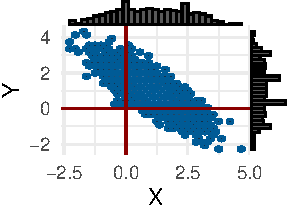
\includegraphics{missing_data_files/figure-beamer/missing_correlated_data-1} \end{center}

\vspace{-0.2in}

\begin{itemize}
\tightlist
\item
  Multiple imputation: simulate datasets from joint distribution, fit
  separately, and combine.
\item
  Bayesian data augmentation: introduce missing data, \(Y_{miss}\) as
  latent variables. Target the joint posterior
  \(\pi(Y_{miss},\theta|Y_{obs})\).
\end{itemize}

\end{frame}

\begin{frame}{Lecture 20 of Statistical Rethinking}
\protect\hypertarget{lecture-20-of-statistical-rethinking-2}{}

\begin{itemize}
\tightlist
\item
  Different missingness mechanisms, MCAR, MAR, and MNAR, require
  different models.
\item
  Imputation can improve precision for estimates of interest
  (shrinkage!).
\item
  Bayesian inference always starts with a \emph{joint} model for data,
  parameters, and covariates.
\end{itemize}

\end{frame}

\begin{frame}{Plan for today}
\protect\hypertarget{plan-for-today}{}

Two examples:

\begin{itemize}
\tightlist
\item
  Model BMI as a function of cholesterol and age.

  \begin{itemize}
  \tightlist
  \item
    Data augmentation with \texttt{brms} (Burkner, 2019).
  \item
    Off-the-shelf, flexible, relatively straightforward syntax.
  \end{itemize}
\item
  Compartmental models for partially observed incidence data.

  \begin{itemize}
  \tightlist
  \item
    Introduce true incidence as a latent variable.
  \item
    Ordinary differential equations describe the latent incidence.
  \end{itemize}
\end{itemize}

\end{frame}

\begin{frame}[fragile]{Example: BMI vs.~Cholesterol}
\protect\hypertarget{example-bmi-vs.cholesterol}{}

Data (\texttt{nhanes} from the \texttt{mice} package)

\begin{itemize}
\tightlist
\item
  18 individuals, omit people missing both BMI and cholesterol.
\item
  BMI (kg/m\(^2\))
\item
  Total serum cholesterol (mg/dL)
\end{itemize}

\begin{verbatim}
##   chl  bmi
## 2 187 22.7
## 3 187   NA
## 5 113 20.4
## 6 184   NA
## 7 118 22.5
## 8 187 30.1
\end{verbatim}

\end{frame}

\begin{frame}{Example: BMI vs.~Cholesterol}
\protect\hypertarget{example-bmi-vs.cholesterol-1}{}

Key features: \vspace{-0.1in}

\begin{itemize}
\tightlist
\item
  Missingness in cholesterol and BMI, we'll assume MAR so need to impute
  but not model missingness (see Statistical Rethinking lecture 20 for
  the explanation of this).
\item
  Looks like higher BMI associated with slightly higher cholesterol.
\end{itemize}

\begin{center}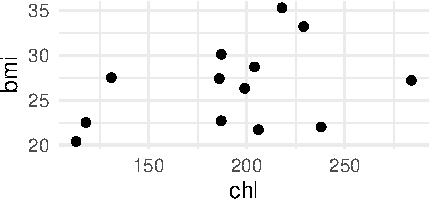
\includegraphics{missing_data_files/figure-beamer/nhanes_plot-1} \end{center}

\end{frame}

\begin{frame}{Example: BMI vs.~Cholesterol}
\protect\hypertarget{example-bmi-vs.cholesterol-2}{}

Model: \vspace{-0.1in}

\[\begin{aligned}
BMI_{obs,i} &\sim LogNormal(\mu_{bmi,i}, \sigma^2_{bmi}) \\
BMI_{miss,i} &\sim LogNormal(\mu_{bmi,i}, \sigma^2_{bmi}) \\
\mu_{bmi,i} &= \beta_0 + \beta_1 CHL_i\\
CHL_{obs,i} &\sim Normal(\mu_{chl}, \sigma^2_{chl}) \\
CHL_{miss,i} &\sim Normal(\mu_{chl}, \sigma^2_{chl}) \\
+\ Priors &\dots
\end{aligned}\]

\begin{itemize}
\tightlist
\item
  MAR \(\implies\) observed and missing variables exchangeable in the
  prior.
\item
  If MNAR, have to model probability of missing given latent value
  (Chapters 8 and 18 of Gelman et al., 2013).
\item
  If we fit this in \texttt{Stan}, declare observed values as data and
  missing values as parameters, which we estimate just like any other
  parameters.
\end{itemize}

\end{frame}

\begin{frame}[fragile]{Interlude: Algorithmic Implementation}
\protect\hypertarget{interlude-algorithmic-implementation}{}

Example - normal means problem with missing values:
\(y_i\sim N(\mu, \sigma^2).\)

\begin{verbatim}
data {
  int<lower=0> N_obs; # number observed
  int<lower=0> N_mis; # number missing
  real y_obs[N_obs];  # vector of observed values
}
\end{verbatim}

\end{frame}

\begin{frame}[fragile]{Interlude: Algorithmic Implementation}
\protect\hypertarget{interlude-algorithmic-implementation-1}{}

Example - normal means problem with missing values:
\(y_i\sim N(\mu, \sigma^2).\)

\begin{verbatim}
parameters {
  real mu;              # mean parameter
  real<lower=0> sigma;  # standard deviation
  real y_mis[N_mis];    # missing values are parameters
}
\end{verbatim}

\end{frame}

\begin{frame}[fragile]{Interlude: Algorithmic Implementation}
\protect\hypertarget{interlude-algorithmic-implementation-2}{}

Example - normal means problem with missing values:
\(y_i\sim N(\mu, \sigma^2).\)

\begin{verbatim}
model {
  # joint distribution for observed and missing variables 
  y_obs ~ normal(mu, sigma); 
  y_mis ~ normal(mu, sigma);
}
\end{verbatim}

\end{frame}

\begin{frame}[fragile]{Example: BMI vs.~Cholesterol}
\protect\hypertarget{example-bmi-vs.cholesterol-3}{}

Trivial to fit using \texttt{brms}:

\begin{Shaded}
\begin{Highlighting}[]
\CommentTok{# model formula, mi() indicates that missing values should be estimated}
\NormalTok{bform <-}\StringTok{ }
\StringTok{    }\KeywordTok{bf}\NormalTok{(bmi }\OperatorTok{|}\StringTok{ }\KeywordTok{mi}\NormalTok{() }\OperatorTok{~}\StringTok{ }\DecValTok{1} \OperatorTok{+}\StringTok{ }\KeywordTok{mi}\NormalTok{(chl), }\DataTypeTok{family =} \StringTok{"lognormal"}\NormalTok{) }\OperatorTok{+}
\StringTok{    }\KeywordTok{bf}\NormalTok{(chl }\OperatorTok{|}\StringTok{ }\KeywordTok{mi}\NormalTok{() }\OperatorTok{~}\StringTok{ }\DecValTok{1}\NormalTok{) }\OperatorTok{+}\StringTok{ }\KeywordTok{set_rescor}\NormalTok{(}\OtherTok{FALSE}\NormalTok{)}

\CommentTok{# call to fit the model}
\NormalTok{nhanes_fit <-}\StringTok{ }\KeywordTok{brm}\NormalTok{(}\DataTypeTok{formula =}\NormalTok{ bform, }
                  \DataTypeTok{data =}\NormalTok{ nhanes,}
                  \DataTypeTok{prior =} \KeywordTok{prior}\NormalTok{(}\KeywordTok{student_t}\NormalTok{(}\DecValTok{3}\NormalTok{,}\DecValTok{0}\NormalTok{,}\DecValTok{5}\NormalTok{), }\DataTypeTok{class =} \StringTok{"b"}\NormalTok{), }\CommentTok{# change priors if you like}
                  \DataTypeTok{refresh =} \DecValTok{0}\NormalTok{) }\CommentTok{# silent compilation and fitting}
\end{Highlighting}
\end{Shaded}

\end{frame}

\begin{frame}{Example: BMI vs.~Cholesterol}
\protect\hypertarget{example-bmi-vs.cholesterol-4}{}

Posterior is full of lines for BMI vs.~cholesterol and values for
cholesterol.

\begin{center}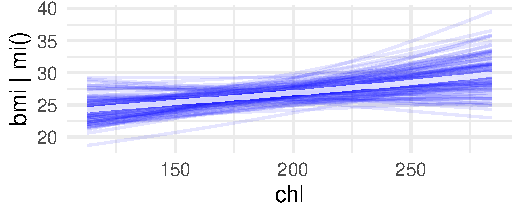
\includegraphics{missing_data_files/figure-beamer/nhanes_marginals-1} \end{center}

\begin{center}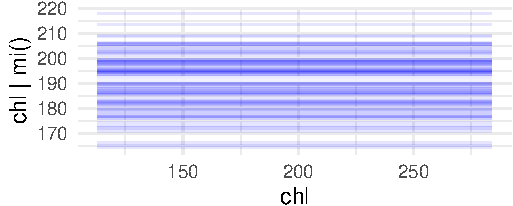
\includegraphics{missing_data_files/figure-beamer/nhanes_marginals-2} \end{center}

\end{frame}

\begin{frame}{Example: BMI vs.~Cholesterol}
\protect\hypertarget{example-bmi-vs.cholesterol-5}{}

Interrogate the posterior predictive distribution to examine fit.

\begin{figure}

{\centering 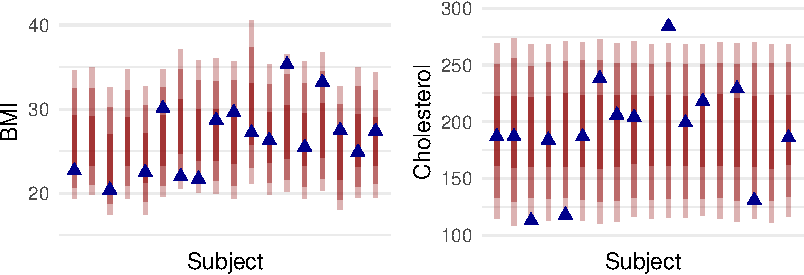
\includegraphics{missing_data_files/figure-beamer/nhanes_postpred-1} 

}

\caption{Posterior predicted BMI and cholesterol.}\label{fig:nhanes_postpred}
\end{figure}

\end{frame}

\begin{frame}{Example: Partially Observed Epidemic Count Data}
\protect\hypertarget{example-partially-observed-epidemic-count-data}{}

Parially observed incidence data: \vspace{-0.1in}

\begin{itemize}
\tightlist
\item
  \(N_{SI}(t_\ell) =\) Cumulative infections up to \(t_\ell\),
\item
  \(Y_\ell =\) new cases seen in \((t_{\ell-1},t_\ell]\),
\item
  \(Y_\ell \sim Neg.Binomial(\mu = \rho\times(N_{SI}(t_\ell) - N_{SI}(t_{\ell-1})),\ \sigma^2 = \mu(1 + \mu / \phi)).\).
\end{itemize}

\begin{center}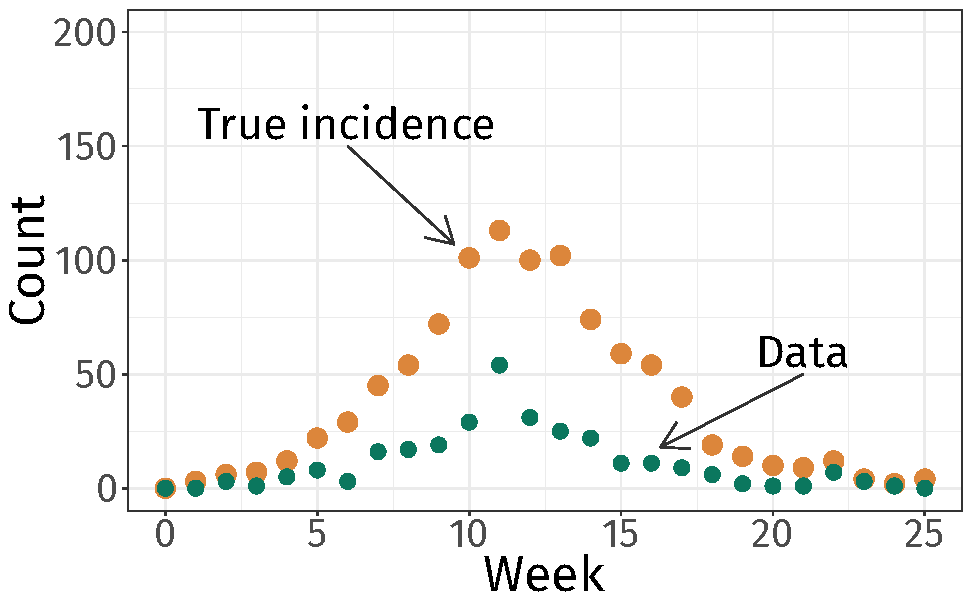
\includegraphics[width=0.5\linewidth]{incid_plot} \end{center}

\end{frame}

\begin{frame}{Example: Partially Observed Epidemic Count Data}
\protect\hypertarget{example-partially-observed-epidemic-count-data-1}{}

\textbf{Important:} \vspace{-0.1in}

\begin{itemize}
\tightlist
\item
  Only observe a \emph{fraction of cases} at \emph{discrete times}.
\item
  Data come from an outbreak that evolves \emph{continuously} in time.
\end{itemize}

\textbf{What do we want to learn?}\vspace{-0.1in}

\begin{itemize}
\tightlist
\item
  How many people were infected? How many people were infected?
\item
  How to characterize the transmission dynamics of the outbreak?
\end{itemize}

\end{frame}

\begin{frame}{Example: Partially Observed Epidemic Count Data}
\protect\hypertarget{example-partially-observed-epidemic-count-data-2}{}

\textbf{What makes this difficult?} \vspace{-0.1in}

\begin{enumerate}
\tightlist
\item
  \emph{Under-reporting:} epidemic process, \(\bf{X}\), only partially
  observed.
\end{enumerate}

\begin{center}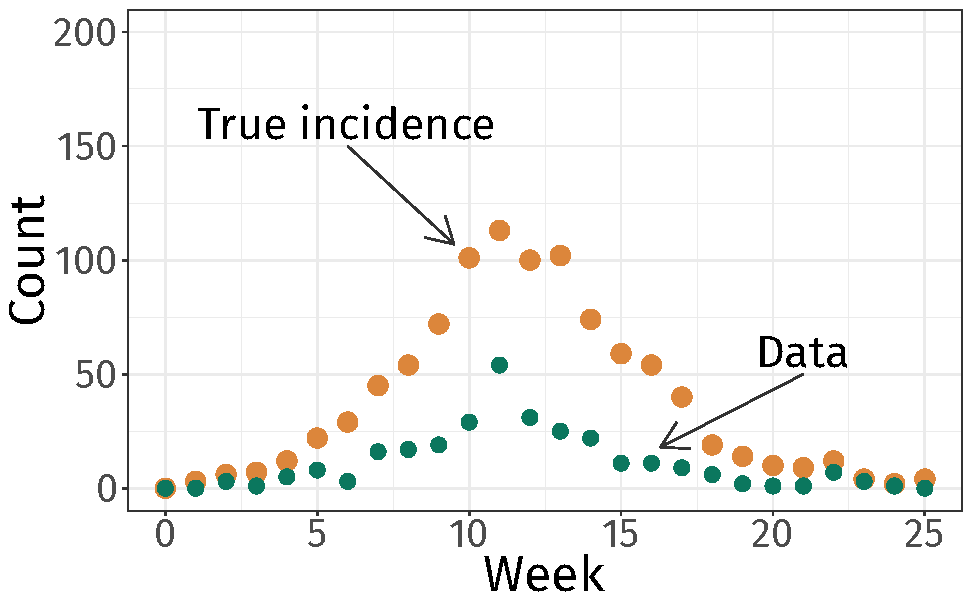
\includegraphics[width=0.3\linewidth]{incid_plot} \end{center}
\vspace{-0.1in}

\begin{enumerate}
\setcounter{enumi}{1}
\item
  \emph{Dependent happenings:} \(\implies\) dependent data,
  \(\bf{Y} = (Y_1,\dots,Y_L)\).

  \begin{itemize}
  \tightlist
  \item
    Observed data likelihood:\vspace{-0.1in}
    \[L(\bf{Y}|\bs{\theta}) = \prod_{\ell=1}^{L}\pi(Y_\ell|Y_1,\dots,Y_{\ell-1},\bs{\theta}) \neq \prod_{\ell=1}^{L}\pi(Y_\ell|\bs{\theta}).\]
  \item
    \emph{Intractable observed data likelihood} State space of
    \(\bf{N}\) is \emph{huge}, even in small populations!\vspace{-0.1in}
    \[L(\bf{Y}|\bs{\theta}) = \int \prod_{\ell = 1}^{L} \pi(Y_\ell|Y_{1},\dots,Y_{\ell-1},\bf{N},\bs{\theta})\pi(\bf{N}|\bs{\theta})d\bf{N}\]\vspace{-0.1in}
  \end{itemize}
\end{enumerate}

\end{frame}

\begin{frame}{Example: Partially Observed Epidemic Count Data}
\protect\hypertarget{example-partially-observed-epidemic-count-data-3}{}

\textbf{Strategy:} \vspace{-0.1in}

\begin{itemize}
\tightlist
\item
  \emph{Bayesian data augmentation} - introduce incident event
  processes, \(\bf{N} = (\bf{N}_{SI},\bf{N}_{IR})\), as latent variables
  in the model.
\item
  Target the joint posterior, \(\pi(\bf{N},\bs{\theta}|\bf{Y})\).
\end{itemize}

\textbf{Challenge:} Need a tractable representation for the transition
density of \(\bf{N}(t_\ell)|\bf{N}(t_{\ell-1}),\bs{\theta}\).
\vspace{-0.1in}

\begin{itemize}
\tightlist
\item
  In large populations, not unreasonable to represent \(\bf{N}\) with a
  deterministic system of ODEs.
\item
  Classical tools in the disease modeling literature, see Allen (2008)
  and Blackwood (2018) for an overview.
\end{itemize}

\end{frame}

\begin{frame}{Example: Partially Observed Epidemic Count Data}
\protect\hypertarget{example-partially-observed-epidemic-count-data-4}{}

\textbf{Deterministic SIR model:}

\begin{minipage}{0.45\linewidth}
Incidence paths are solutions to systems of differential equations,
$$\footnotesize\begin{aligned}
\frac{\rmd}{\rmd t}\left(\begin{array}{l}
N_{SI} \\
N_{IR}
\end{array}\right) &= \left(\begin{array}{c}
\beta SI \\
\mu I
\end{array}\right), \\ 
&= \left(\begin{array}{c}
\beta (S_0 - N_{SI})(I_0 + N_{SI} - N_{IR}) \\
\mu (I_0 + N_{SI} - N_{IR})
\end{array}\right),
\end{aligned}$$
subject to $\bf{X}_0 = (S_0,I_0,R_0),\ \bf{N}_0 = \bs{0}.$

\begin{itemize}
\item $\beta$ = per-contact infection rate.
\item $\mu$ = recovery rate.
\item Priors on $1/\mu$ = mean infectious period and $\mathcal{R}_0 = \beta N / \mu =$ basic reproduction number. 
\end{itemize}

\end{minipage}\hfill
\begin{minipage}{0.45\linewidth}

\begin{center}
\includegraphics[width=0.9\linewidth]{sir_diagram} \end{center}


\begin{center}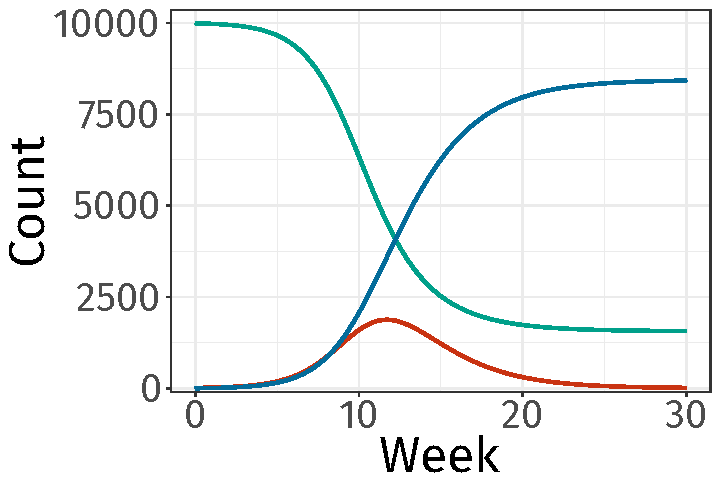
\includegraphics[width=1\linewidth]{sir_ode} \end{center}
\end{minipage}

\end{frame}

\begin{frame}{Example: Partially Observed Epidemic Count Data}
\protect\hypertarget{example-partially-observed-epidemic-count-data-5}{}

Joint model, \(\pi(\bf{Y},\bf{N},\bs{\theta})\), where \(\bf{N}\) has
the \emph{Markov} property. \vspace{-0.1in}

\begin{itemize}
\tightlist
\item
  Data, \(\bf{Y}\), are conditionally independent given \(\bf{N}\).
\item
  \emph{Simplified complete data likelihood:}\vspace{-0.1in}
  \[L(\bf{Y},\bf{N} | \bs{\theta}) = \pi(\bf{N}(t_0)|\bs{\theta})\prod_{\ell = 1}^L \textcolor{RoyalBlue}{\pi(Y_\ell|\bf{N}(t_\ell),\bs{\theta})} \textcolor{BrickRed}{\pi(\bf{N}(t_\ell) | \bf{N}(t_{\ell-1}),\bs{\theta})}. \vspace{-0.15in}\]

  \begin{itemize}
            \item $\textcolor{RoyalBlue}{\pi(Y_\ell|\bf{N}(t_\ell),\bs{\theta})}$ --- sampling model, negative binomial.
            \item $\textcolor{BrickRed}{\pi(\bf{N}(t_\ell) | \bf{N}(t_{\ell-1}),\bs{\theta})}$ --- transition density for latent epidemic, SIR
        \end{itemize}
\item
  Here, \(\bs{\theta}\) maps 1:1 onto \(\bf{N}\) so no need to sample
  \(\bf{N}\) explicitly.
\item
  Stochastic representations of \(\bf{N}\) require sampling latent
  paths. Tradeoff realism and compuational tractability.
\end{itemize}

\textbf{Key point:} true incidence is missing data. In the Bayesian
paradigm we estimate it like any other parameter by including it in our
joint model and targeting the posterior!

\end{frame}

\begin{frame}{Example: Partially Observed Epidemic Count Data}
\protect\hypertarget{example-partially-observed-epidemic-count-data-6}{}

\textbf{Goal:} Infer
\(\pi(\bs{\theta},\bf{N}|\bf{Y}) \propto L(\bf{Y}|\bf{N},\bs{\theta})\pi(\bf{N}|\bs{\theta})\pi(\bs{\theta})\).

\begin{itemize}
\item \textcolor{BrickRed}{\textbf{Outbreak dynamics:}} $\pi(\bf{N}|\bs{\theta})$
    
        
        \begin{center}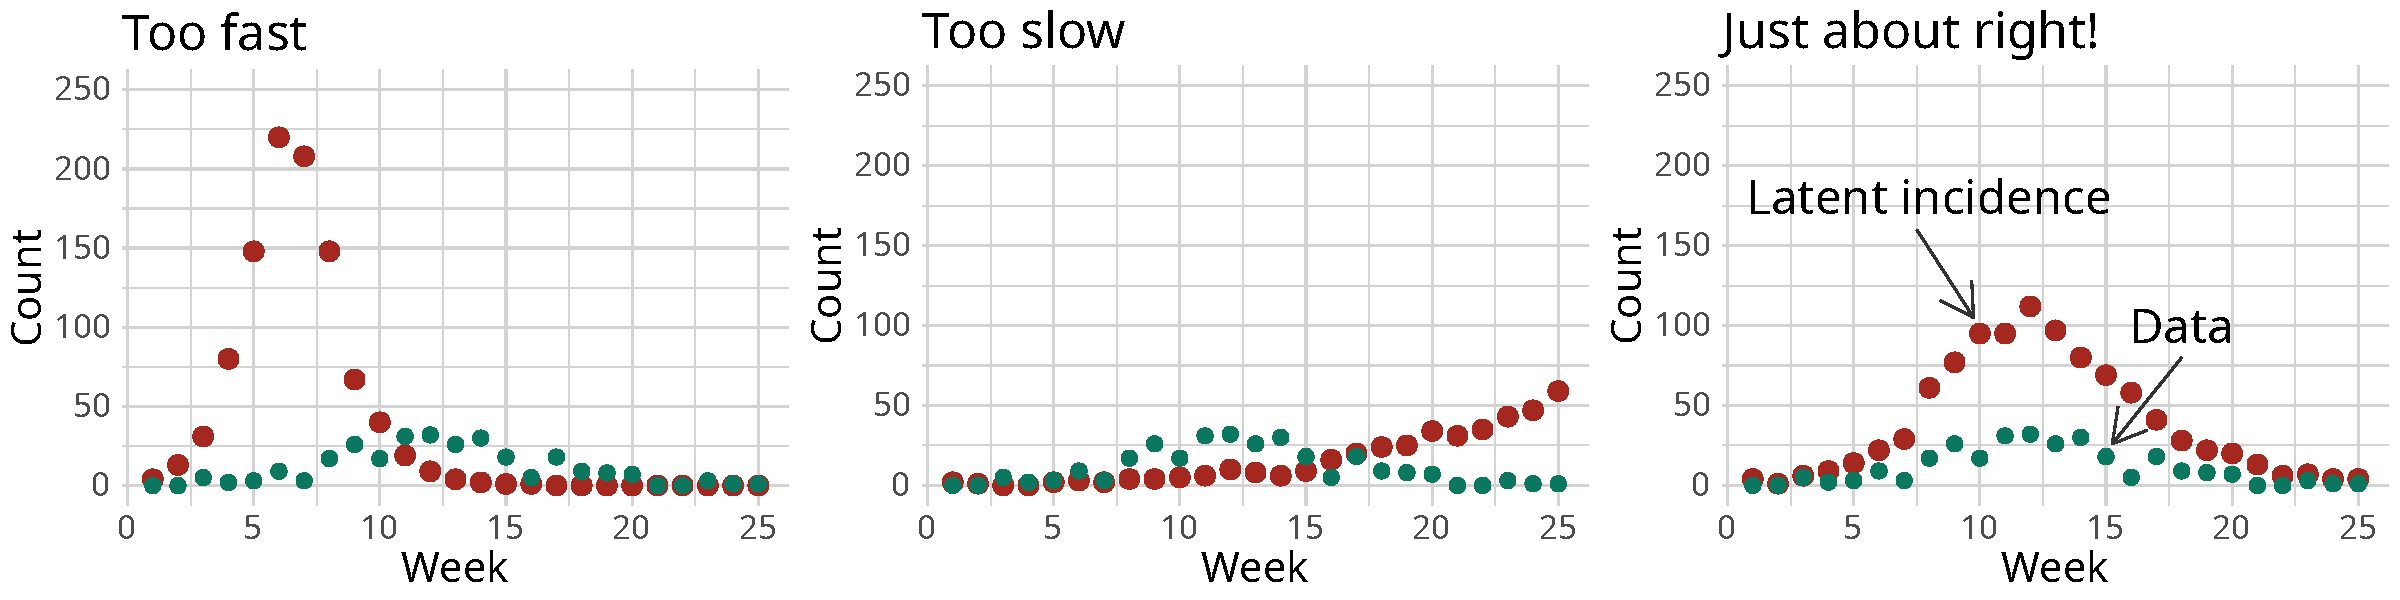
\includegraphics[width=0.9\linewidth]{sim_dynamics_plots} \end{center}
\item \textcolor{RoyalBlue}{\textbf{Observation model:}} $L(\bf{Y}|\bf{N},\bs{\theta})$
    
        
        \begin{center}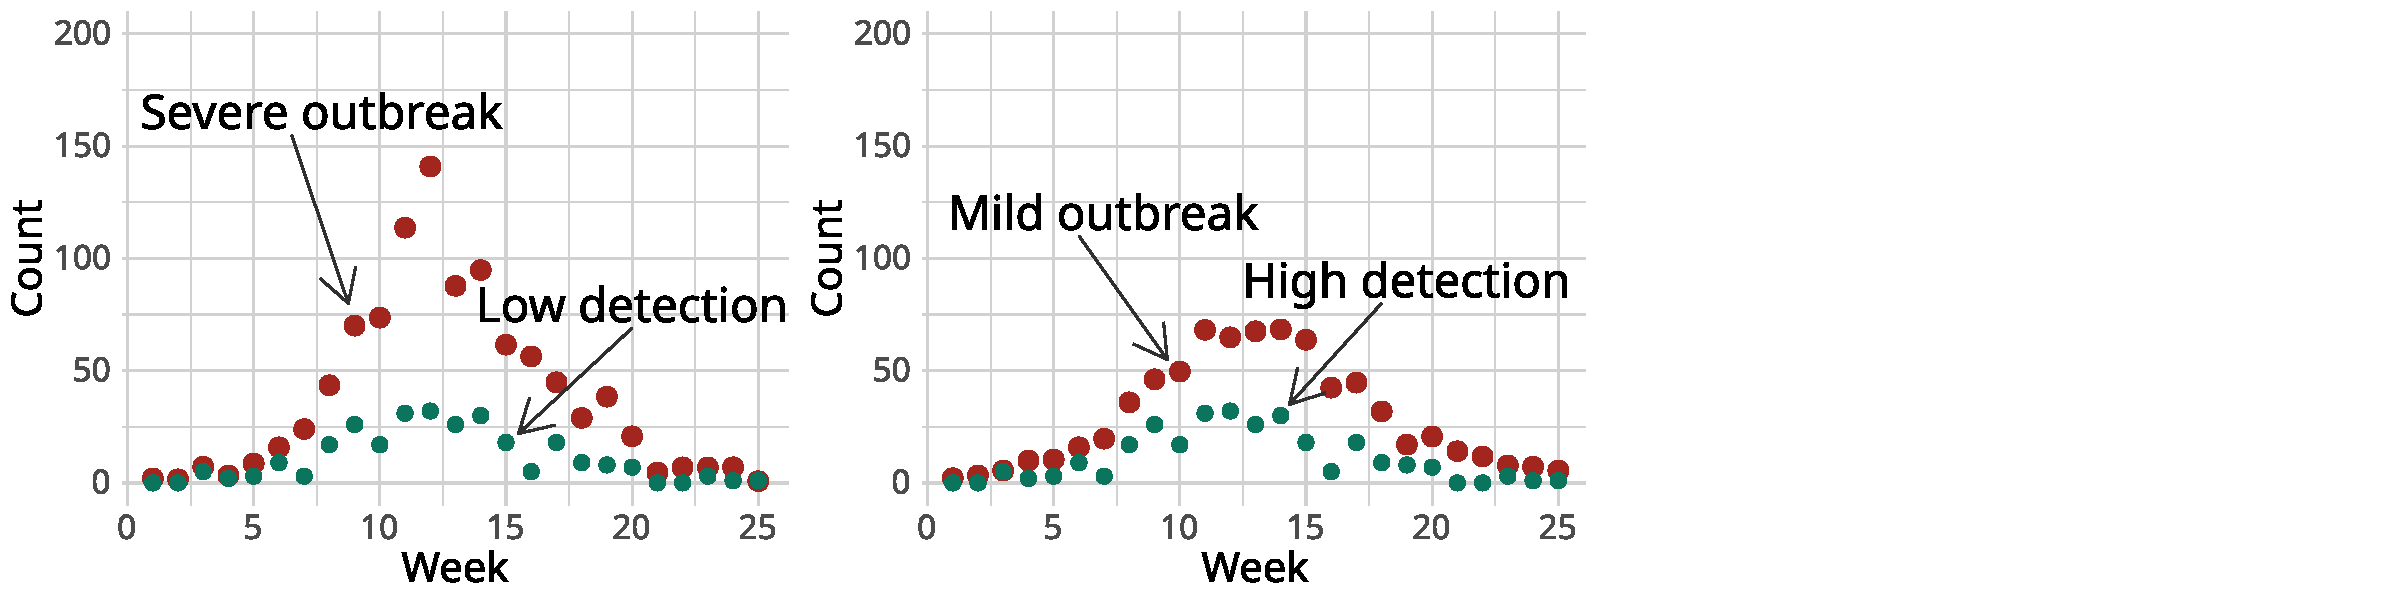
\includegraphics[width=0.9\linewidth]{latent_high_low_dist1} \end{center}
\end{itemize}

\end{frame}

\begin{frame}{Example: Partially Observed Epidemic Count Data}
\protect\hypertarget{example-partially-observed-epidemic-count-data-7}{}

\textbf{Goal:} Infer
\(\pi(\bs{\theta},\bf{N}|\bf{Y}) \propto L(\bf{Y}|\bf{N},\bs{\theta})\pi(\bf{N}|\bs{\theta})\pi(\bs{\theta})\).

\begin{itemize}
\item \textcolor{BrickRed}{\textbf{Outbreak dynamics:}} $\pi(\bf{N}|\bs{\theta})$
    
        
        \begin{center}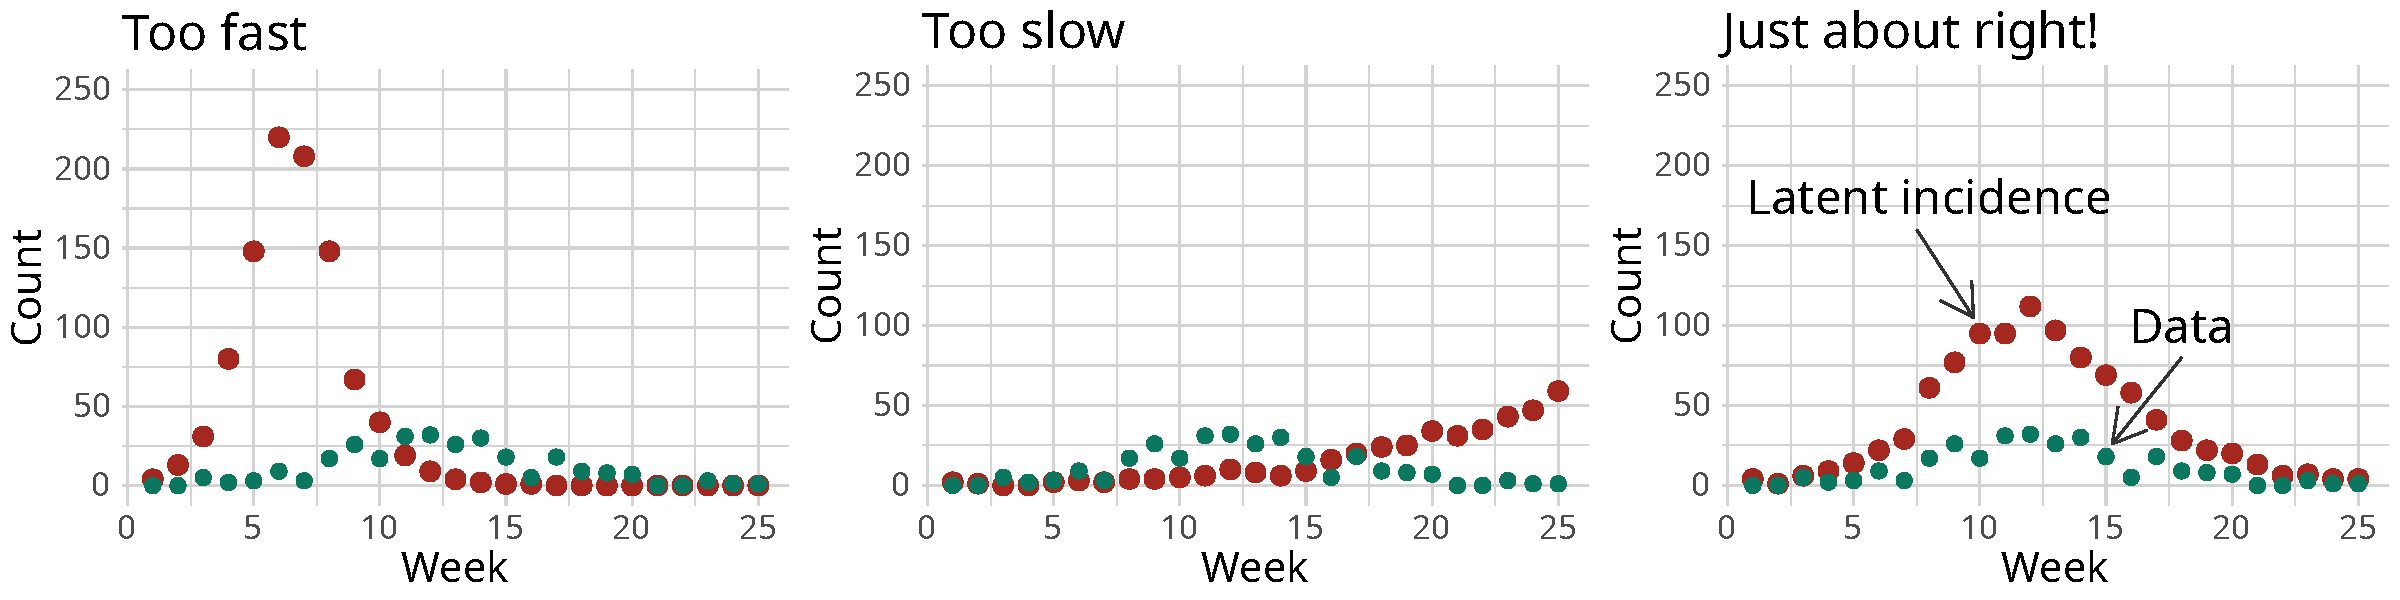
\includegraphics[width=0.9\linewidth]{sim_dynamics_plots} \end{center}
\item \textcolor{RoyalBlue}{\textbf{Observation model:}} $L(\bf{Y}|\bf{N},\bs{\theta})$
    
        
        \begin{center}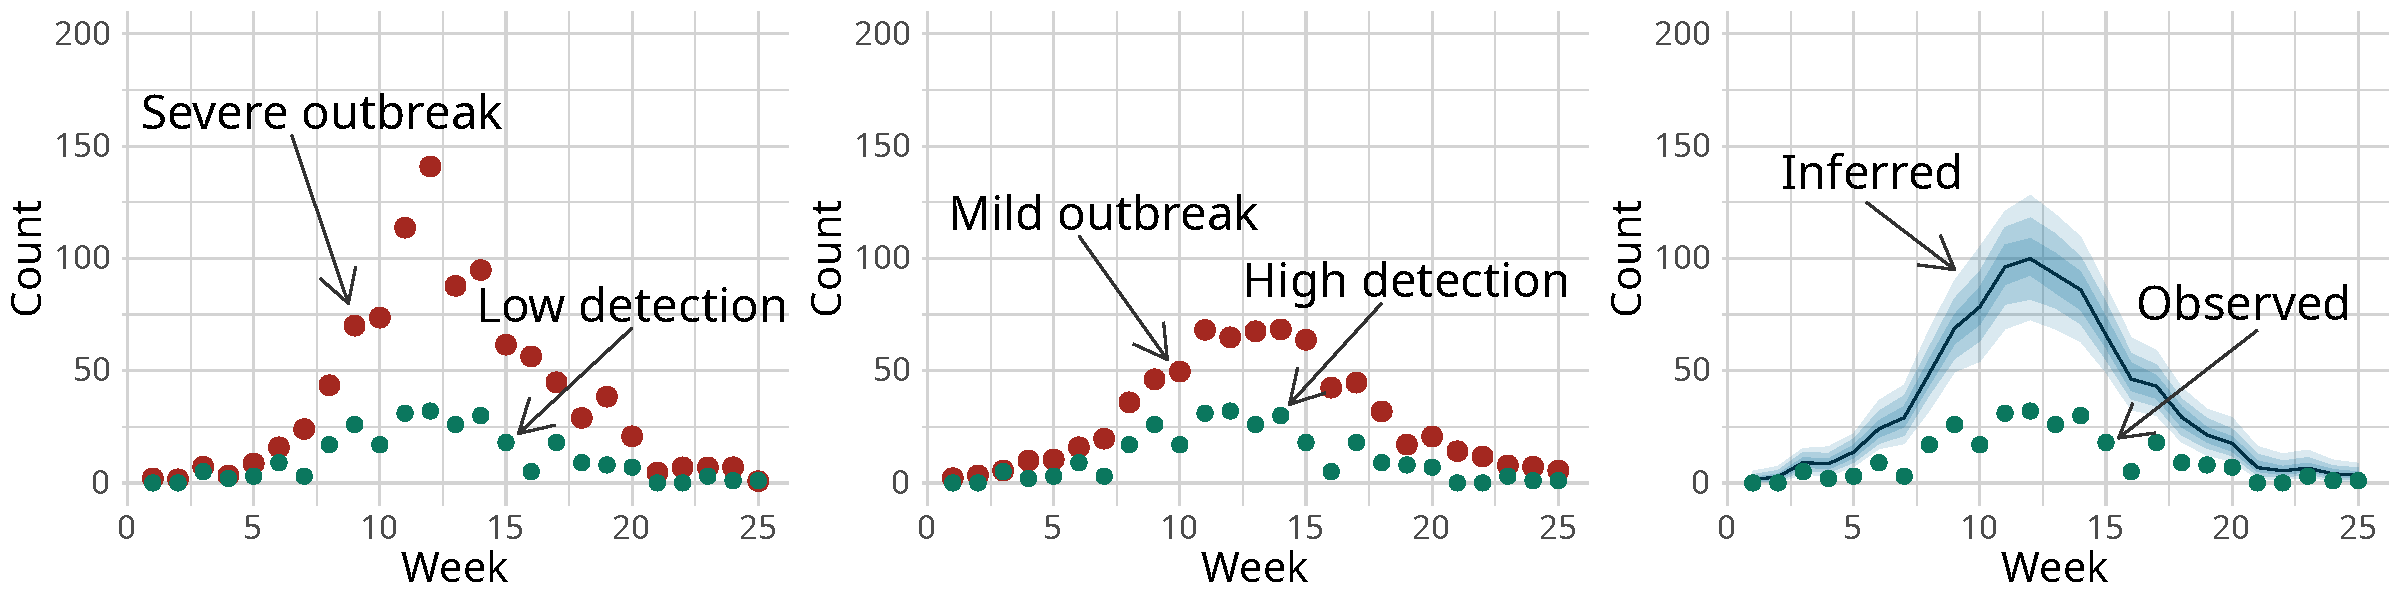
\includegraphics[width=0.9\linewidth]{latent_high_low_dist2} \end{center}
\end{itemize}

\end{frame}

\begin{frame}{Example: Partially Observed Epidemic Count Data}
\protect\hypertarget{example-partially-observed-epidemic-count-data-8}{}

\textbf{Goal:} Infer
\(\pi(\bs{\theta},\bf{N}|\bf{Y}) \propto L(\bf{Y}|\bf{N},\bs{\theta})\pi(\bf{N}|\bs{\theta})\pi(\bs{\theta})\).

\begin{itemize}
\item \textcolor{BrickRed}{\textbf{Outbreak dynamics:}} $\pi(\bf{N}|\bs{\theta})$
    
        
        \begin{center}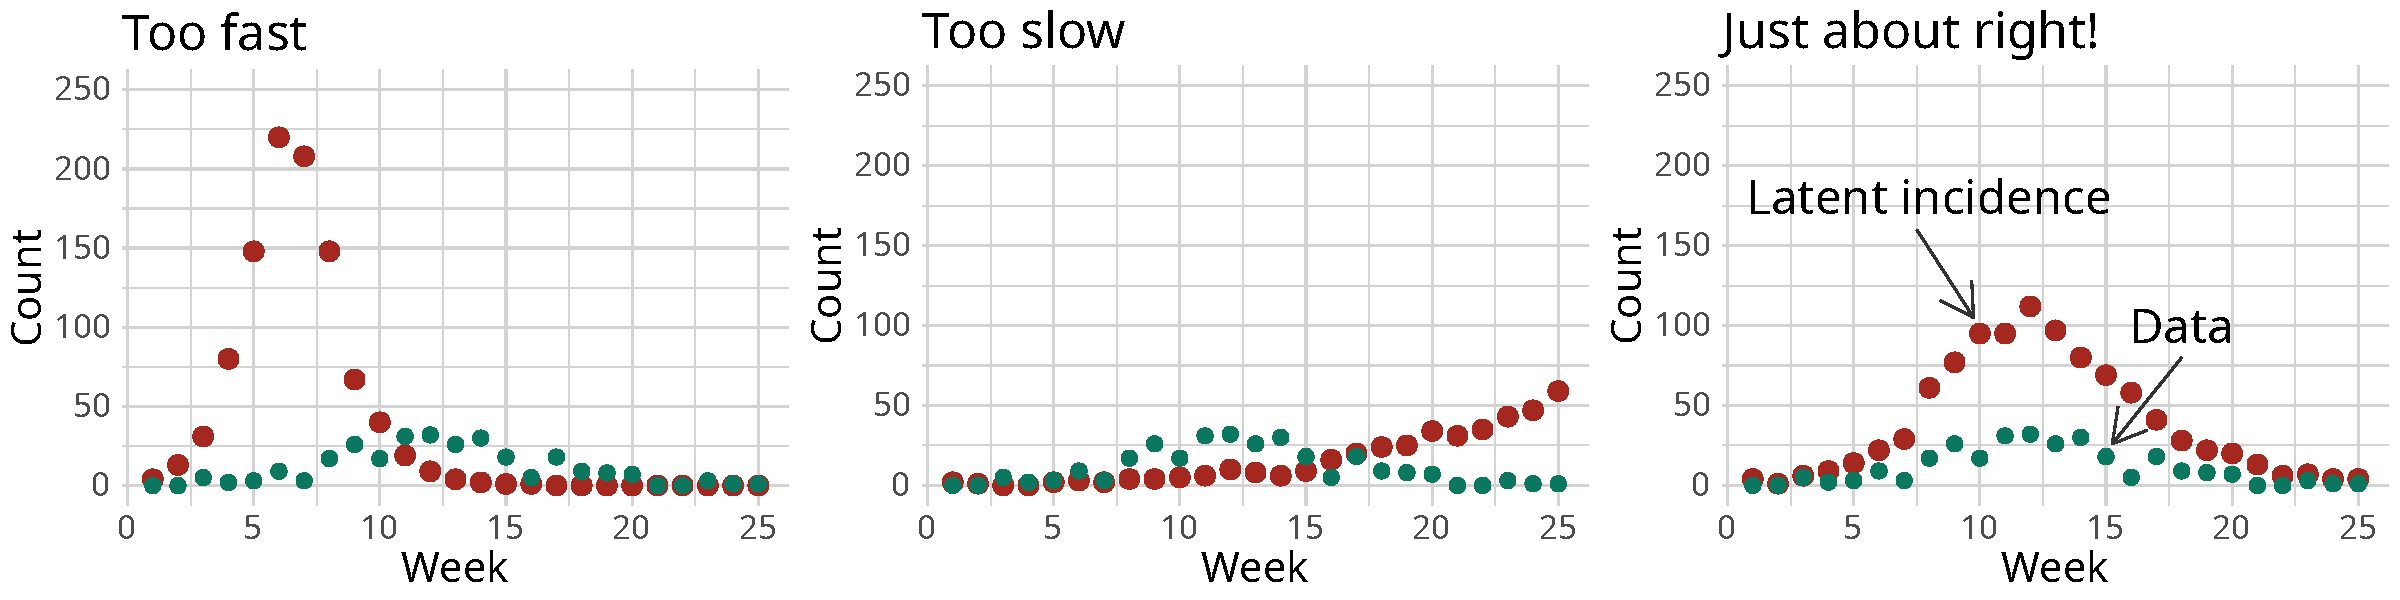
\includegraphics[width=0.9\linewidth]{sim_dynamics_plots} \end{center}
\item \textcolor{RoyalBlue}{\textbf{Observation model:}} $L(\bf{Y}|\bf{N},\bs{\theta})$
    
        
        \begin{center}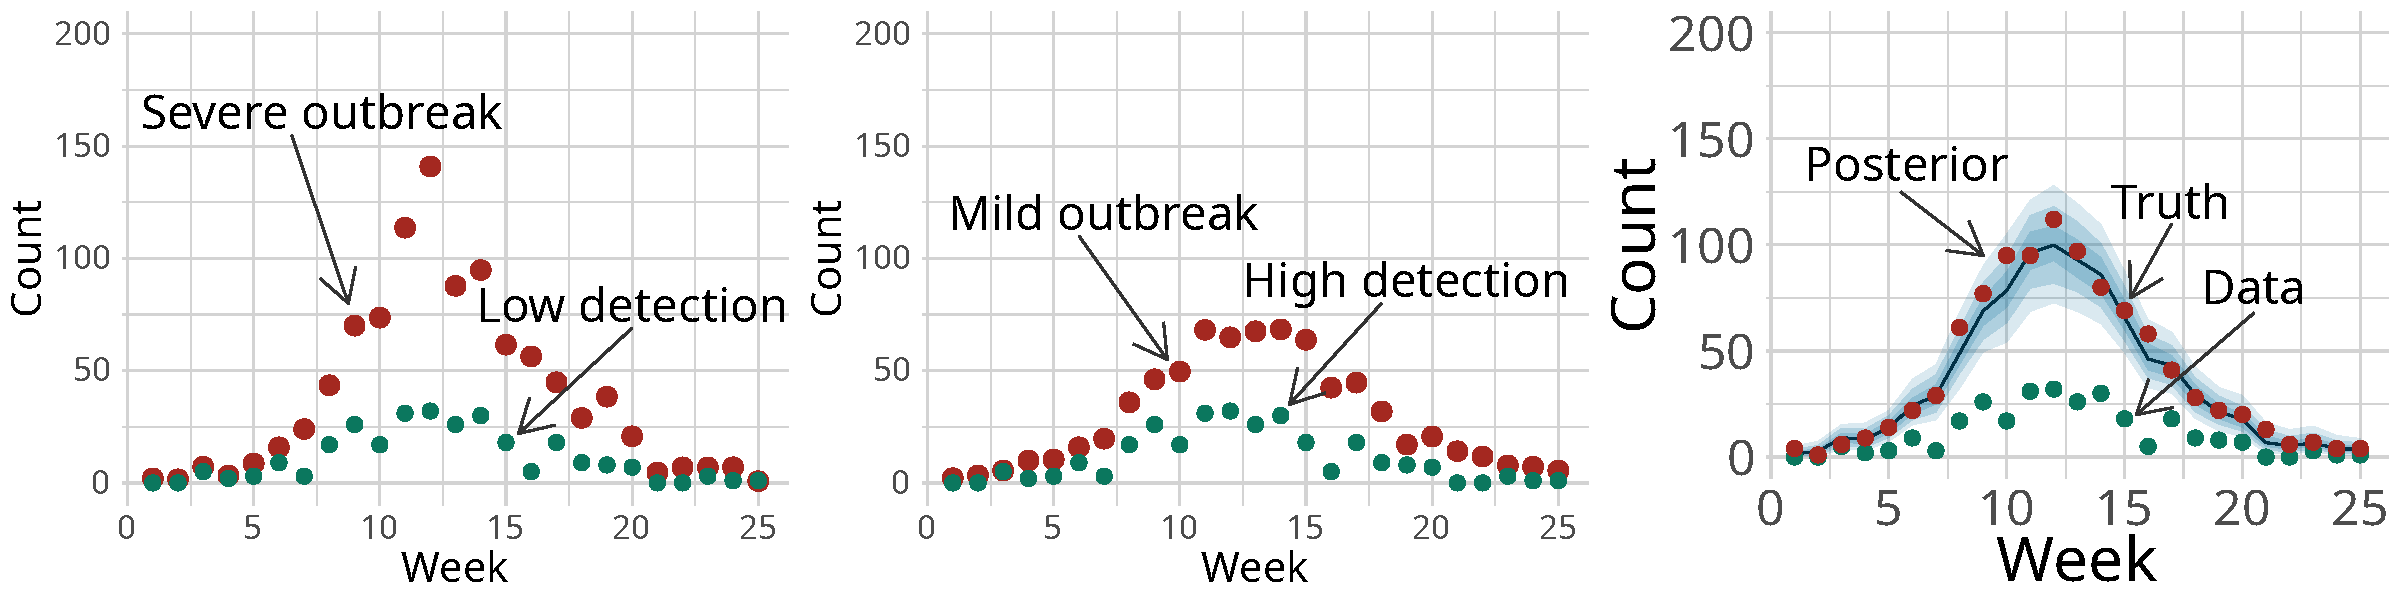
\includegraphics[width=0.9\linewidth]{latent_high_low_truth} \end{center}
\end{itemize}

\end{frame}

\begin{frame}{Example: Partially Observed Epidemic Count Data}
\protect\hypertarget{example-partially-observed-epidemic-count-data-9}{}

Posterior distributions of model parameters:

\begin{center}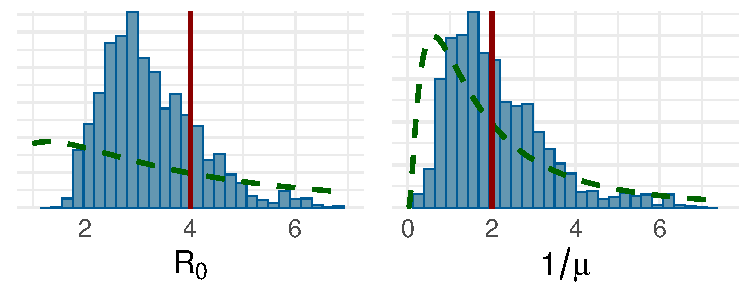
\includegraphics[width=0.6\linewidth]{sir_posts} \end{center}

\end{frame}

\begin{frame}{Wrapping up}
\protect\hypertarget{wrapping-up}{}

\begin{itemize}
\tightlist
\item
  Quantify two kinds of uncertainty, epistemic, which reflects
  subjective ignorance, and aleatory, which is uncertainty due to
  chance.
\item
  A Bayesian model \textbf{always} defines a joint distribution for data
  and parameters.
\item
  Some simple examples, PREVAIL II and linear regression; some complex
  hierarchical models and missing data.
\item
  Failure modes of misspecified priors under poorly chosen scales,
  weakly informative priors as a reasonable strategy.
\item
  Good workflow is like going to the dentist.
\item
  Various computational tools.
\end{itemize}

\end{frame}

\begin{frame}{References}
\protect\hypertarget{references}{}

Allen, Linda JS. ``An introduction to stochastic epidemic models.''
Mathematical epidemiology. Springer, Berlin, Heidelberg, 2008. 81-130.

Blackwood, Julie C., and Lauren M. Childs. ``An introduction to
compartmental modeling for the budding infectious disease modeler.''
\emph{Letters in Biomathematics} 5.1 (2018): 195-221.

P. Burkner. ``Handle Missing Values with brms.''
\url{https://cran.r-project.org/web/packages/brms/vignettes/brms_missings.html}
(2019).

Gelman, Andrew, et al.~Bayesian data analysis. Chapman and Hall/CRC,
2013.

\end{frame}

\begin{frame}{}
\protect\hypertarget{section}{}

\end{frame}

\end{document}